% Made up for the tikra benchmark.
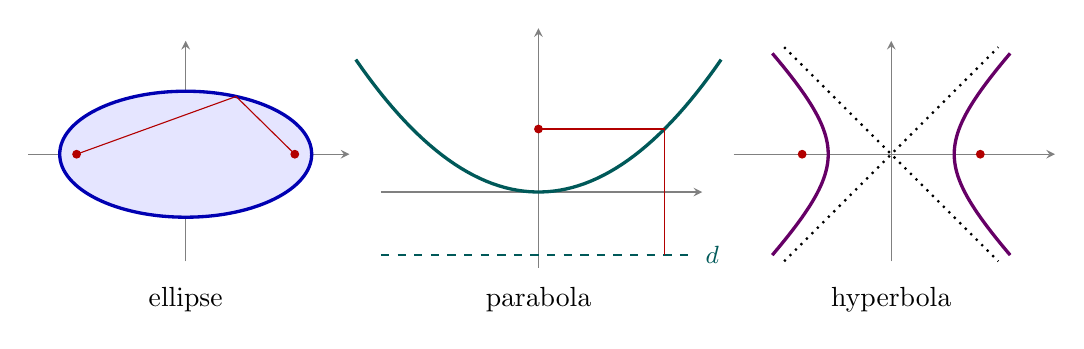
\begin{tikzpicture}[scale=0.8, >=stealth]
  \tikzset{ax/.style={->, gray}, focus/.style={fill=red!70!black}, curve/.style={very thick}}
  % ellipse x^2/4 + y^2 = 1
  \begin{scope}
    \draw[ax] (-2.5,0) -- (2.6,0); \draw[ax] (0,-1.7) -- (0,1.8);
    \draw[curve, blue!70!black, fill=blue!10] (0,0) ellipse (2 and 1);
    \fill[focus] (-1.732,0) circle (2pt) (1.732,0) circle (2pt);
    \draw[red!70!black] (-1.732,0) -- (0.8,0.9165) -- (1.732,0);
    \node at (0,-2.3) {ellipse};
  \end{scope}
  % parabola y = x^2/4, focus (0,1), directrix y = -1
  \begin{scope}[xshift=5.6cm, yshift=-0.6cm]
    \draw[ax] (-2.5,0) -- (2.6,0); \draw[ax] (0,-1.2) -- (0,2.6);
    \draw[curve, teal!70!black, domain=-2.9:2.9, samples=60] plot (\x, {\x*\x/4});
    \draw[dashed, teal!70!black] (-2.5,-1) -- (2.5,-1) node[right, font=\small] {$d$};
    \fill[focus] (0,1) circle (2pt);
    \draw[red!70!black] (0,1) -- (2,1) -- (2,-1);
    \node at (0,-1.7) {parabola};
  \end{scope}
  % hyperbola x^2 - y^2 = 1
  \begin{scope}[xshift=11.2cm]
    \draw[ax] (-2.5,0) -- (2.6,0); \draw[ax] (0,-1.7) -- (0,1.8);
    \draw[dotted, thick] (-1.7,-1.7) -- (1.7,1.7) (-1.7,1.7) -- (1.7,-1.7);
    \draw[curve, violet!80!black, domain=-1.25:1.25, samples=50]
      plot ({cosh(\x)}, {sinh(\x)}) plot ({-cosh(\x)}, {sinh(\x)});
    \fill[focus] (-1.414,0) circle (2pt) (1.414,0) circle (2pt);
    \node at (0,-2.3) {hyperbola};
  \end{scope}
\end{tikzpicture}
